% !TeX TXS-program:compile = txs:///pdflatex/[--shell-escape]

\documentclass[11pt, letterpaper]{article}

\usepackage[utf8]{inputenc}
\usepackage[T1]{fontenc}
\usepackage{lmodern}
\usepackage{graphicx}
\usepackage{longtable}
\usepackage{wrapfig}
\usepackage{rotating}
\usepackage{amsmath}
\usepackage{textcomp}
\usepackage{amssymb}
\usepackage{hyperref}
\usepackage[spanish]{babel}
\usepackage[round]{natbib}
\usepackage{subcaption}

\title{\bfseries Tarea}
\author{Ángel García Báez}
\date{\today}
\setcounter{tocdepth}{4} 

\begin{document}
	% Página de presentación
	\begin{titlepage}
		\centering
		
\includegraphics[width=0.2\textwidth]{logo.png}\par
		\vspace{1cm}
		{\LARGE \bfseries Universidad Veracruzana \par}
		\vspace{1cm}
		{\Large Maestría en Inteligencia Artificial\par}
		\vspace{3cm}
		{\LARGE \bfseries Lógica difusa \par}
		\vspace{1cm}
		{\Large \bfseries Tarea 13. Problema del mesero con 3 variables usando lógica difusa tipo II en python con la librería pyit2fls. \par}
		\vfill
		{\Large \textit{Ángel García Báez}\par}
		\vfill
		{\Large Dr. Sergio Hernández Méndez \par}
		\vfill
		{\Large \today \par}
	\end{titlepage}
	
	% Página exclusiva para la tabla de contenidos
	\newpage
	\tableofcontents
	\newpage
	
% Explicación breve

\section{Introducción}

En el presente reporte se explica brevemente la expansión del problema del mesero vista en la tarea 2 y 3, a una versión donde se hacen uso de 3 variables de entrada junto con un sistema de lógica difusa tipo 2 para determinar la propina del mesero.

Se llevo a cabo la elaboración del sistema en el lenguaje de programación Python y haciendo uso de la librería de codigo abierto pyit2fls \cite{haghrah2025pyit2fls}.


\newpage


\section{Problema del mesero con 3 variables}

\subsection{Explicación del Problema}

Se tiene el problema de determinar cuanta propina dejarle a un mesero en un restaurante después de comer. Para ello, se toman en cuenta las variables de Servicio, la comida y el lugar.

Para trasladar esto a un sistema difuso, se especifican a continuación los valores de las variables, el universo del discurso y las funciones de membresía.


\subsection{Variables y sus codificaciones}

A continuación se listan los valores de las variables lingüísticas que se
propusieron para SERVICIO, COMIDA, LUGAR y PROPINA como sigue:

\begin{enumerate}
	\item Servicio: Malo ($\mu = 0$, $\sigma = [2.5,2]$), Regular ($\mu = 5$, $\sigma = [2,1.5]$) y Bueno ($\mu = 8$, $\sigma = [3,2]$).
	\begin{figure}[h]
		\centering
		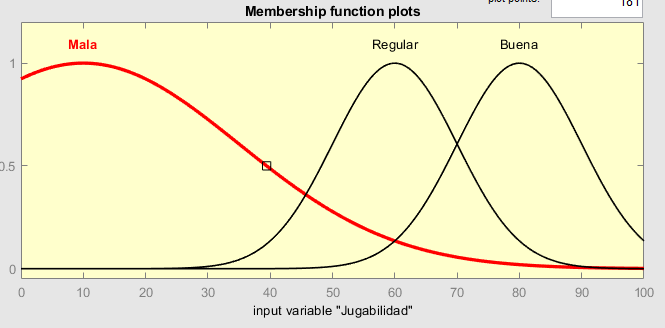
\includegraphics[width=0.8\textwidth]{IMG/P11.png}
	\end{figure}
	
	\newpage
	
	\item Comida: Malo ($\mu = 1$, $\sigma = [2.5,2]$), Normal ($\mu = 5$, $\sigma = [2.5,2]$), Buena ($\mu = 7$, $\sigma = [2,1.5]$) y Excelente ($\mu = 9$, $\sigma = [3,2]$).
	\begin{figure}[h]
		\centering
		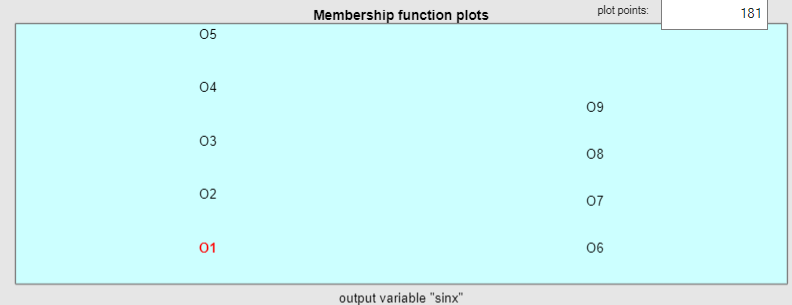
\includegraphics[width=0.8\textwidth]{IMG/P12.png}
	\end{figure}

	\item Lugar: Malo ($\mu = 0$, $\sigma = [3,2]$), Aceptable ($\mu = 3.5$, $\sigma = [2.5,2]$), Agradable ($\mu = 6$, $\sigma = [2,1.5]$) y Excelente ($\mu = 9$, $\sigma = [3,2]$).
\begin{figure}[h]
	\centering
	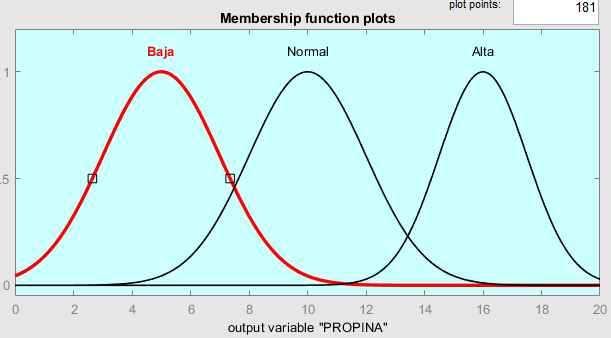
\includegraphics[width=0.8\textwidth]{IMG/P13.png}
\end{figure}

	\newpage
	
	\item Propina: Pésima ($\mu = 0$, $\sigma = [3,2.5]$), Baja ($\mu = 7$, $\sigma = [4, 3]$), Regular ($\mu = 13$, $\sigma = [4,3]$) y Alta ($\mu = 19$, $\sigma = [3,2]$).
	\begin{figure}[h]
		\centering
		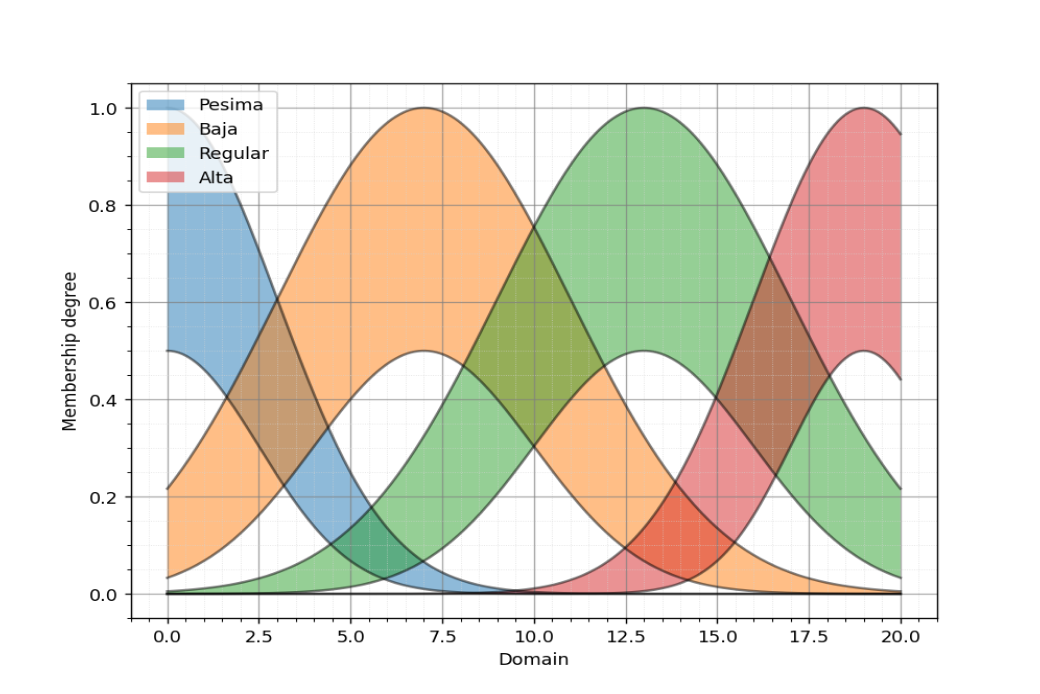
\includegraphics[width=0.8\textwidth]{IMG/P14.png}
	\end{figure}
\end{enumerate}

Considerando que se está trabajando con un sistema difuso tipo II, es necesario especificar tanto la función de membresía que se encuentra en un rango superior, como la que se encuentra en un rango inferior. Por simplicidad, se optó por usar funciones de membresía Gaussianas en donde la función de membresía superior tiene una desviación estándar mayor que la función de membresía inferior, compartiendo la misma media. Tambien cabe mencionar que se le asigno un valor de 1 a la función superior y un valor de 0.5 a la función inferior para que la huella difusa fuera alta.

Para aplicar la parte del sistema de logica tipo 2, se siguio acorde a la documentación de \cite{haghrah2025pyit2fls} y de lo mencionado en el articulo de \cite{lu_genetic-algorithm-based_2015}, de donde se menciona que se aplican 2 sistemas, un sistema clásico mandhami para las inferencias pero con un reductor de tipo basado en el algoritmo de Karnik-Mendel.


\newpage

\subsection{Reglas de inferencia.}

A continuación se muestran las treinta y dos reglas que se construyeron para este problema:

\begin{enumerate}
	\item R1: Si \textbf{SERVICIO} es \textbf{\textit{BUENO}}, la \textbf{COMIDA} es \textbf{\textit{BUENA}} y el \textbf{LUGAR} es \textbf{\textit{ACEPTABLE}}, la \textbf{PROPINA} es \textbf{\textit{REGULAR}}.
	\item R2: Si \textbf{SERVICIO} es \textbf{\textit{BUENO}}, la \textbf{COMIDA} es \textbf{\textit{BUENA}} y el \textbf{LUGAR} es \textbf{\textit{AGRADABLE}}, la \textbf{PROPINA} es \textbf{\textit{ALTA}}.
	\item R3: Si \textbf{SERVICIO} es \textbf{\textit{BUENO}}, la \textbf{COMIDA} es \textbf{\textit{BUENA}} y el \textbf{LUGAR} es \textbf{\textit{EXCELENTE}}, la \textbf{PROPINA} es \textbf{\textit{ALTA}}.
	\item R4: Si \textbf{SERVICIO} es \textbf{\textit{BUENO}}, la \textbf{COMIDA} es \textbf{\textit{BUENA}} y el \textbf{LUGAR} es \textbf{\textit{MALO}}, la \textbf{PROPINA} es \textbf{\textit{REGULAR}}.
	\item R5: Si \textbf{SERVICIO} es \textbf{\textit{BUENO}}, la \textbf{COMIDA} es \textbf{\textit{EXCELENTE}} y el \textbf{LUGAR} es \textbf{\textit{AGRADABLE}}, la \textbf{PROPINA} es \textbf{\textit{ALTA}}.
	\item R6: Si \textbf{SERVICIO} es \textbf{\textit{BUENO}}, la \textbf{COMIDA} es \textbf{\textit{EXCELENTE}} y el \textbf{LUGAR} es \textbf{\textit{EXCELENTE}}, la \textbf{PROPINA} es \textbf{\textit{ALTA}}.
	\item R7: Si \textbf{SERVICIO} es \textbf{\textit{BUENO}}, la \textbf{COMIDA} es \textbf{\textit{MALA}} y el \textbf{LUGAR} es \textbf{\textit{ACEPTABLE}}, la \textbf{PROPINA} es \textbf{\textit{BAJA}}.
	\item R8: Si \textbf{SERVICIO} es \textbf{\textit{BUENO}}, la \textbf{COMIDA} es \textbf{\textit{MALA}} y el \textbf{LUGAR} es \textbf{\textit{AGRADABLE}}, la \textbf{PROPINA} es \textbf{\textit{BAJA}}.
	\item R9: Si \textbf{SERVICIO} es \textbf{\textit{BUENO}}, la \textbf{COMIDA} es \textbf{\textit{MALA}} y el \textbf{LUGAR} es \textbf{\textit{EXCELENTE}}, la \textbf{PROPINA} es \textbf{\textit{BAJA}}.
	\item R10: Si \textbf{SERVICIO} es \textbf{\textit{BUENO}}, la \textbf{COMIDA} es \textbf{\textit{MALA}} y el \textbf{LUGAR} es \textbf{\textit{MALO}}, la \textbf{PROPINA} es \textbf{\textit{BAJA}}.
	\item R11: Si \textbf{SERVICIO} es \textbf{\textit{BUENO}}, la \textbf{COMIDA} es \textbf{\textit{NORMAL}} y el \textbf{LUGAR} es \textbf{\textit{ACEPTABLE}}, la \textbf{PROPINA} es \textbf{\textit{REGULAR}}.
	\item R12: Si \textbf{SERVICIO} es \textbf{\textit{BUENO}}, la \textbf{COMIDA} es \textbf{\textit{NORMAL}} y el \textbf{LUGAR} es \textbf{\textit{AGRADABLE}}, la \textbf{PROPINA} es \textbf{\textit{REGULAR}}.
	\item R13: Si \textbf{SERVICIO} es \textbf{\textit{BUENO}}, la \textbf{COMIDA} es \textbf{\textit{NORMAL}} y el \textbf{LUGAR} es \textbf{\textit{EXCELENTE}}, la \textbf{PROPINA} es \textbf{\textit{ALTA}}.
	\item R14: Si \textbf{SERVICIO} es \textbf{\textit{BUENO}}, la \textbf{COMIDA} es \textbf{\textit{NORMAL}} y el \textbf{LUGAR} es \textbf{\textit{MALO}}, la \textbf{PROPINA} es \textbf{\textit{REGULAR}}.
	\item R15: Si \textbf{SERVICIO} es \textbf{\textit{MALO}}, la \textbf{COMIDA} es \textbf{\textit{MALA}} y el \textbf{LUGAR} es \textbf{\textit{ACEPTABLE}}, la \textbf{PROPINA} es \textbf{\textit{PÉSIMA}}.
	\item R16: Si \textbf{SERVICIO} es \textbf{\textit{MALO}}, la \textbf{COMIDA} es \textbf{\textit{MALA}} y el \textbf{LUGAR} es \textbf{\textit{AGRADABLE}}, la \textbf{PROPINA} es \textbf{\textit{BAJA}}.
	\item R17: Si \textbf{SERVICIO} es \textbf{\textit{MALO}}, la \textbf{COMIDA} es \textbf{\textit{MALA}} y el \textbf{LUGAR} es \textbf{\textit{EXCELENTE}}, la \textbf{PROPINA} es \textbf{\textit{BAJA}}.
	\item R18: Si \textbf{SERVICIO} es \textbf{\textit{MALO}}, la \textbf{COMIDA} es \textbf{\textit{MALA}} y el \textbf{LUGAR} es \textbf{\textit{MALO}}, la \textbf{PROPINA} es \textbf{\textit{PÉSIMA}}.
	\item R19: Si \textbf{SERVICIO} es \textbf{\textit{MALO}}, la \textbf{COMIDA} es \textbf{\textit{NORMAL}} y el \textbf{LUGAR} es \textbf{\textit{ACEPTABLE}}, la \textbf{PROPINA} es \textbf{\textit{BAJA}}.
	\item R20: Si \textbf{SERVICIO} es \textbf{\textit{MALO}}, la \textbf{COMIDA} es \textbf{\textit{NORMAL}} y el \textbf{LUGAR} es \textbf{\textit{AGRADABLE}}, la \textbf{PROPINA} es \textbf{\textit{BAJA}}.
	\item R21: Si \textbf{SERVICIO} es \textbf{\textit{REGULAR}}, la \textbf{COMIDA} es \textbf{\textit{BUENA}} y el \textbf{LUGAR} es \textbf{\textit{ACEPTABLE}}, la \textbf{PROPINA} es \textbf{\textit{REGULAR}}.
	\item R22: Si \textbf{SERVICIO} es \textbf{\textit{REGULAR}}, la \textbf{COMIDA} es \textbf{\textit{BUENA}} y el \textbf{LUGAR} es \textbf{\textit{AGRADABLE}}, la \textbf{PROPINA} es \textbf{\textit{REGULAR}}.
	\item R23: Si \textbf{SERVICIO} es \textbf{\textit{REGULAR}}, la \textbf{COMIDA} es \textbf{\textit{EXCELENTE}} y el \textbf{LUGAR} es \textbf{\textit{ACEPTABLE}}, la \textbf{PROPINA} es \textbf{\textit{REGULAR}}.
	\item R24: Si \textbf{SERVICIO} es \textbf{\textit{REGULAR}}, la \textbf{COMIDA} es \textbf{\textit{EXCELENTE}} y el \textbf{LUGAR} es \textbf{\textit{EXCELENTE}}, la \textbf{PROPINA} es \textbf{\textit{ALTA}}.
	\item R25: Si \textbf{SERVICIO} es \textbf{\textit{REGULAR}}, la \textbf{COMIDA} es \textbf{\textit{EXCELENTE}} y el \textbf{LUGAR} es \textbf{\textit{MALO}}, la \textbf{PROPINA} es \textbf{\textit{REGULAR}}.
	\item R26: Si \textbf{SERVICIO} es \textbf{\textit{REGULAR}}, la \textbf{COMIDA} es \textbf{\textit{MALA}} y el \textbf{LUGAR} es \textbf{\textit{ACEPTABLE}}, la \textbf{PROPINA} es \textbf{\textit{BAJA}}.
	\item R27: Si \textbf{SERVICIO} es \textbf{\textit{REGULAR}}, la \textbf{COMIDA} es \textbf{\textit{MALA}} y el \textbf{LUGAR} es \textbf{\textit{AGRADABLE}}, la \textbf{PROPINA} es \textbf{\textit{BAJA}}.
	\item R28: Si \textbf{SERVICIO} es \textbf{\textit{REGULAR}}, la \textbf{COMIDA} es \textbf{\textit{MALA}} y el \textbf{LUGAR} es \textbf{\textit{EXCELENTE}}, la \textbf{PROPINA} es \textbf{\textit{BAJA}}.
	\item R29: Si \textbf{SERVICIO} es \textbf{\textit{REGULAR}}, la \textbf{COMIDA} es \textbf{\textit{MALA}} y el \textbf{LUGAR} es \textbf{\textit{MALO}}, la \textbf{PROPINA} es \textbf{\textit{PÉSIMA}}.
	\item R30: Si \textbf{SERVICIO} es \textbf{\textit{REGULAR}}, la \textbf{COMIDA} es \textbf{\textit{NORMAL}} y el \textbf{LUGAR} es \textbf{\textit{AGRADABLE}}, la \textbf{PROPINA} es \textbf{\textit{REGULAR}}.
	\item R31: Si \textbf{SERVICIO} es \textbf{\textit{REGULAR}}, la \textbf{COMIDA} es \textbf{\textit{NORMAL}} y el \textbf{LUGAR} es \textbf{\textit{EXCELENTE}}, la \textbf{PROPINA} es \textbf{\textit{REGULAR}}.
	\item R32: Si \textbf{SERVICIO} es \textbf{\textit{REGULAR}}, la \textbf{COMIDA} es \textbf{\textit{NORMAL}} y el \textbf{LUGAR} es \textbf{\textit{MALO}}, la \textbf{PROPINA} es \textbf{\textit{REGULAR}}.
\end{enumerate}

\newpage

\subsection{Gráficos del problema del mesero}

A continuación se muestran 2 gráficas de superficie, una es el resultado de dejar fija la variable lugar en 0 y la otra es el resultado de dejar la variable Servicio en 10:

\begin{figure}[h]
	\centering
	\begin{subfigure}{0.9\textwidth} % Reducido de 0.45
		\centering
		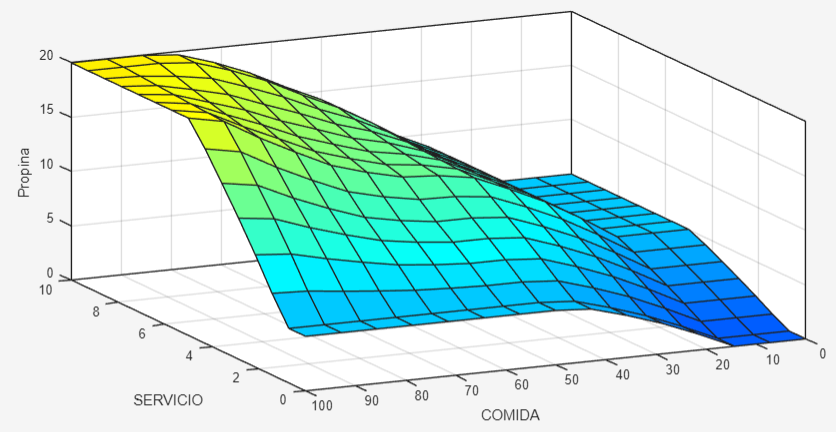
\includegraphics[width=1\textwidth]{IMG/P15.png}
		\label{fig:G1}
	\end{subfigure}
	\hfill
	\begin{subfigure}{0.8\textwidth} % Reducido de 0.45
		\centering
		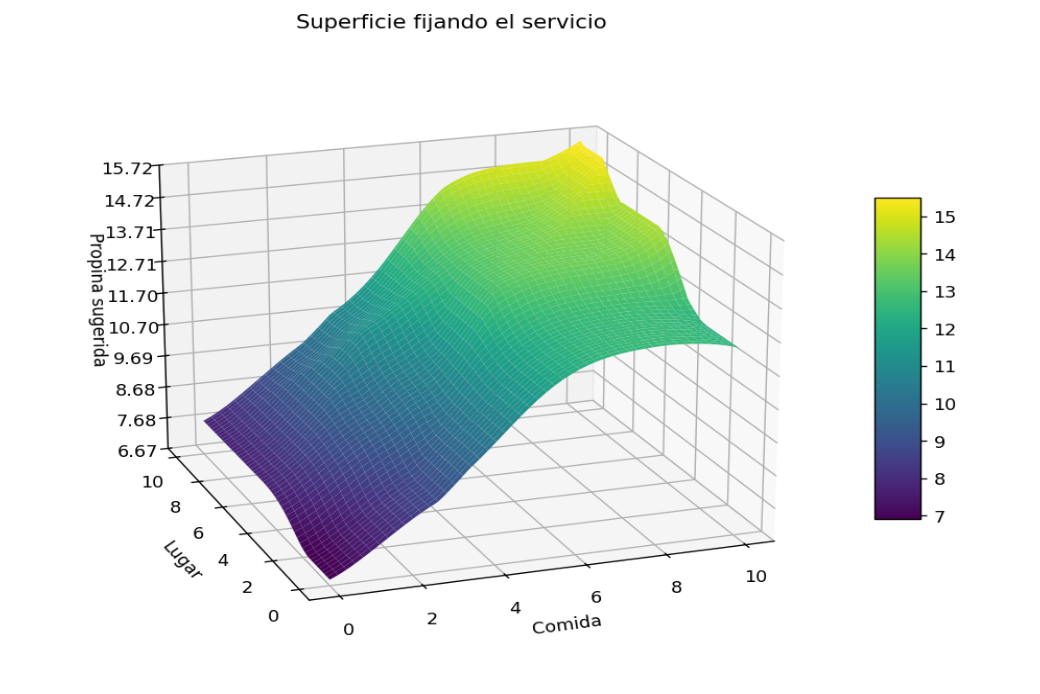
\includegraphics[width=0.9\textwidth]{IMG/P16.png}
		\label{fig:G2}
	\end{subfigure}
	\label{fig:comparacion1}
\end{figure}

La gráfica producida muestra un comportamiento suave sin llegar a tocar los extremos de la propina (0 y 20).



\newpage

\subsection{Corridas de prueba: Casos mínimo, medio y máximo}

Con la finalidad de probar el sistema, se hicieron 3 corridas para verificar los resultados.
La corrida minima consta de dejar todos los valores de las variables en 0, la corrida media deja todos los valores de las variables en 5 y la corrida maxima deja todos los valores de las variables en 10.


\begin{figure}[h]
	\centering
	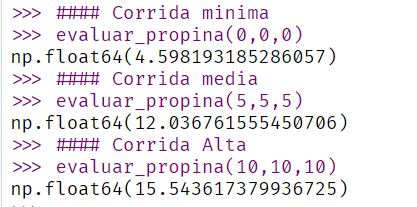
\includegraphics[width=0.7\linewidth]{IMG/P17}
	\caption{}
	\label{fig:h1}
\end{figure}


\newpage

\section{Conclusiones}

El trabajar con un sistema de logica difusa tipo 2 abre las puertas a incorporar de forma más amplia el manejo de lo difuso entre las variables dentro de las funciones de membresia. Si bien, el sistema da buenos resultados, no es capaz de llegar a los máximos, por lo que es necesario definir de forma muy clara las funciones de membresia. Así mismo, una contra encontrada durante la experimentación, fue que la obtención de los valores CRISP puede llegar a volverse computacionalmente costosa, debido a que por cada valor CRISP es necesario primero hacer el procesado de las entradas y hacer la reducción de tipos con KMA, lo que le exige trabajo extra al programa.




\newpage

\section{Referencias}

\bibliographystyle{apalike}  % Estilo de cita, puedes cambiarlo si lo prefieres.
\bibliography{Biblio}         % Aquí incluyes el archivo .bib (sin extensión).

\newpage

\section{Anexos}

Este reporte se envía con los códigos anexos que corresponden a:

\begin{enumerate}
	\item El archivo en .py que corresponde a mi sistema. 


\end{enumerate}



\end{document}

